\subsection{Motivation}
\begin{frame}{\phantom{title}}
	\begin{center}
		%\enquote{Everyone knows that debugging is twice as hard as writing a program in the first place. \\[1.5em] So if you're as clever as you can be when you write it, how will you ever debug it?} \\[3em]
		%-- Brian Kernighan in ``The Elements of Programming Style''

		\begin{figure}
			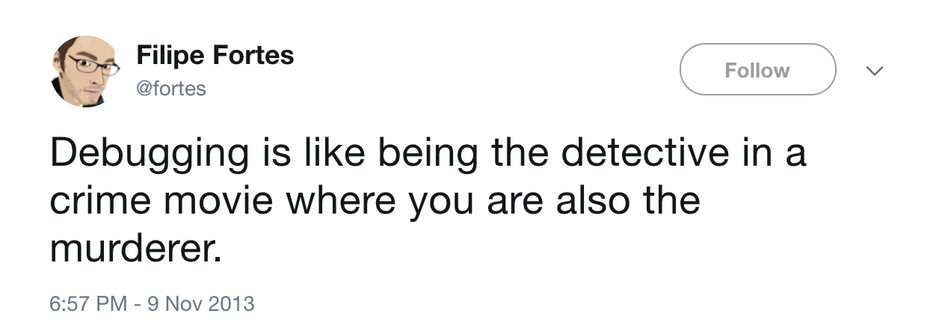
\includegraphics[width= \textwidth]{../figures/tweet-quote.png}
		\end{figure}

	\end{center}
\end{frame}


\subsection{Idea}
%\begin{frame}{Version Control allows DD}
%	\begin{itemize}
%		\item Version Control has been around since the 80's
%		\item central terms: configuration, change
%	\end{itemize}
%\end{frame}

\begin{frame}{The DD idea}
	\begin{columns}
		\begin{column}{0.4\textwidth}
			\begin{center}
			Configuration:\\[2em]

			\yd\\[1em]
			Passes tests. \green{\cmark}
			\end{center}
		\end{column}
		\begin{column}{0.2\textwidth}
			\begin{center}
			Changes:\\[1.5em]
			$\longrightarrow$ \\
			$\longrightarrow$ \\
			$\longrightarrow$ \\
			\end{center}
			
		\end{column}
		\begin{column}{0.4\textwidth}
			\begin{center}	
			Configuration:\\[2em]

			\td\\[1em]
			Tests fail. \red{\xmark}
			\end{center}
		\end{column}
	\end{columns}

	\bigskip

	\begin{exampleblock}{Idea: Delta Debugging}
		Find the minimal set of changes between \yd and \td that induces the failure.
	\end{exampleblock}
\end{frame}

\subsection{First approach}

\begin{frame}{A first approach}
	\begin{itemize}
		\item $\C = \set{\Delta_1, \dots, \Delta_n}$ : All changes between \yd and \td
		\item $c \subseteq \C$ : A configuration (set of changes applied to \yd)
		\item $test: 2^{\C} \to \set{\cmark,\xmark,\qmark}$ : Result of the tests applied to a configuration
	\end{itemize}
	
	\bigskip

	A simple binary search can be conducted to find singular failure inducing changes:\\[.5em]

	\begin{algorithmic}[1]
		\Function{simpledd}{$c: 2^{\C}$}
			\If{$|c| = 1$} \Return $c$ \EndIf
			\State Split $c$ into two halves $c_1$, $c_2$ so that $c_1 \cap c_2 = \emptyset$
			\If{($test(c_1) = \xmark$)} \Return $simpledd(c_1)$ \Else{} \Return $simpledd(c_2)$
			\EndIf
		\EndFunction
	\end{algorithmic}
\end{frame}

